\documentclass[a4wide]{article}
\usepackage{a4wide}
\usepackage{graphicx}
\usepackage{float}
\usepackage{hyperref}
\newcommand{\comment}[1]{{\tt #1}}

%opening
\title{}
\author{}

\begin{document}
\begin{titlepage}
\begin{center}


% Oberer Teil der Titelseite:

\textsc{\LARGE Shared Apartments Web Application}\\[1.0cm]
\textsc{\Large Team 8}\\[1.5cm]
% Title
\newcommand{\HRule}{\rule{\linewidth}{0.5mm}}
\HRule \\[0.4cm]
{ \huge \bfseries Software Requirements Specification}\\[0.4cm]

\HRule \\[1.5cm]

% Author and supervisor
\begin{minipage}{0.4\textwidth}
\begin{flushleft} \large
\emph{Developers:}\\
Michael \textsc{Gr\"unig}\\
Sara \textsc{Peeters}\\
Daniel \textsc{Ziltener}
\end{flushleft}
\end{minipage}
\hfill
\begin{minipage}{0.4\textwidth}
\begin{flushright} \large
\emph{Customer:} \\
Haidar \textsc{Osman}
\end{flushright}
\end{minipage}
\\[1.5cm]
\begin{tabular}{|l|l|l|}
\hline
\textbf{Version}&\textbf{Date}&\textbf{Revision description}\\ \hline
0.1 & 22/10/2014 & First SRS in Latex, Requirements Specification, Prototyping (Fluid UI) \\ \hline
0.2 & 29/10/2014 & Persona (Security), User Profile; ads simple create, view  \\ \hline
0.3 & 05/11/2014 & Apartment and Shared Apart: new, view, edit; simple search, timeslots, message Entity\\ \hline
1.0 & 12/11/2014 & v1 Release,some refactoring, Logo and banner, Tests\\ \hline

1.1 & 19/11/2014 & cross-reviewing of team 3\\ \hline

1.2 & 27/11/2014 & Admin Panel, new layout\\ \hline
1.3 & 03/12/2014 & Roommate, Picture Upload, Messeging, Bookmarks, better Layout, Ad-tags  \\ \hline

1.4 & 09/12/2014 & Removal of Admin-Panel, more search options, code cleaning  \\ \hline
2.0 & 10/12/2014 &  v2 Release \\ \hline
\end{tabular}

\vfill

% Unterer Teil der Seite
{\large \today}

\end{center}

\end{titlepage}

\tableofcontents
\clearpage
\section{Introduction}
\subsection{Purpose}
This Software Requirements Specifications (SRS) are the main reference document concerning the Shared Apartments Web Application Rentr. Principle reading parties of the document are the customer (Haydar Osman), and Team 8: Michael Grünig, Sara Peeters and Daniel Ziltener, the developers.

Written in a language understandable for all parties, it aims at giving a complete overview of the project, as currently agreed on. To this end, terms acronyms and abbreviations required to properly interpret the SRS are declared under the Definitions subsection of this section. Furthermore this introductory section contains a quick overview of the project stakeholders, as well as the system under development. A complete list of references to further documents used in the project is also provided.

In the second section functional and non-functional requirements are enlisted. As for the functional requirements we provide a detailed definition list of the main components. How the components will interact is not described in this section. Therefore we refer to the use cases in section 3. We aim to keep this list complete, unambiguous and the requirements verifiable. Requirements will be ordered to priority.

The third section provides an in-depth overview of the system under development from a user point of view. Use cases are schematically represented and described in detail. Also user characteristics are analyzed and described in this section.


The developers commit to updating the document after each customer-meeting, assuring that it represents the project specifications in the best possible way at any time. The customer commits to report mistakes and unclarities in the document to the developers, so that these can be corrected.

\subsection{Stakeholders}
\begin{description}
\item[The customer]is the ordering party in this contract.  He will own and operate the web application after development. 
\item[A Client] of the web application is a internet user who registers to use the services provided by the web application developed.
\end{description}
\subsection{Definitions}
\textit{There are no definitions or abbreviations in this section yet. If any of the terms used in the document are unclear, please notify us, so it can be added to this section.}
\subsection{System goals}
To have the best features of the three pages listed: \\
wgzimmer.ch, \\
students.ch/wohnen \\
and tutti.ch/bern/immobilien/wg-zimmer.

\subsection{System overview}
The system consists of a client-side website and a server-side application containing all the logic, using Java EE as the platform, the Spring Framework for structure, Spring Data together with MySQL for data storage, JSF for webpage structure and Persona as authentication framework.

Users have to log in to the website using Persona and create a profile. Users can then create ads or search for ads. Searches can be stored as alerts, and the user gets notified whenever a new ad is placed matching the criteria. Ad placers can place dates for visits where other users can subscribe. They can also manage visits and enquiries on the webpage. E-Mail-notifications are available.
The administrator can modify and delete users and ads.

\subsubsection{current state and location}
After compiling the web-app can be found at \href{https://localhost:8443/}{https://localhost:8443/}.\\
Currently implemented usecases are: 
\begin{itemize}
\item As a user I want to place an ad for advertising a room in a shared apartment
\item As a user I want to search for relevant ads in a specific area
\item As a user I want to get exhaustive information about a room (e.g. pictures, location, roommate profiles, ..)
\end{itemize}

\subsection{References}
\textit{There are no external references yet. They will be added to this section as needed.}
\section{Specific requirements and definitions}
\subsection{System element definitions}
\subsubsection{Profile}
Each normal user has a profile. 
A profile consists of 2 parts: An obligatory part and an optional part.
Each element contained in a user profile is either visible (V) to other users, or not ().

Obligatory profile:
\begin{itemize}
\item (V) Name
\item (V) Surname
\item () Email address
\item () Password
\item (V) Sex
\item (V) Age
\item () Email options for search alerts (always (default), daily digest, weekly digest, no email)
\item () Email options for reactions on ads (always (default), daily digest, weekly digest, no email)
\item () Email options for other occasions (always (default), daily digest, weekly digest,  no email)
\end{itemize}
Optional profile:
\begin{itemize}
\item (V) profile picture
\item (V) Description
\end{itemize}
\subsubsection{Ad}
Ads are an important component of the web application. 
Some, but not all elements of an ad are searchable (S),
which means that a search can in some way select for this criterium.
\begin{itemize}
\item () Title
\item (S) Address

	Note: address consists of Street, number, ZIP-code and city. ZIP-code is searchable.
\item (S) Category (shared apartment or apartment)
\item (S) Price

	Note: Price is searchable via a from-to-field.
\item (S) Room size

	Note: searchable via a from-to-field.
\item (S) Free from Date

	Note: searchable by indicating a date and one of the options (strict, or earlier, or later).
\item (S) Free until

	Note: can be unlimited, or a date
	is searchable by indicating no limit or a date and one of the options (strict, or earlier, or later).
\item (S) Languages spoken
\item (S) Keywords

	Note: Keywords help to personalize a search, without getting lost in the different terms 
	that can be used for the same thing in a description.
	They are selected from a list.
	Some examples: Vegetarian/Vegan, Non-vegetarian, Quiet neighbourhood, Party-zone, 
	Shared garden/Balcony, bike parking, staying weekends, eating/cooking together...
\item () Pictures
\item () Description
\item (S) Roommates

	Note: Searchable on sex (all male, all female, no preference).
	Searchable on age via a from-to-field.
	Number of roommates is searchable via a from-to-field.
\item () response method: enquiry and/or timeschedule 
\item () Deactivated
\end{itemize}
\subsection{Non-functional requirements}
\begin{itemize}
\item Secure login and data
    User should confirm registration through email link.
    Captcha is used in registration form.
    passwords must have a minimum length 
    maximum number of  login attempts from the same IP. 
\item Logging
    All site traffic is logged in different log files, documenting each user action.
\item Responsive design
    The website adapts to mobile users (smartphones and tablets).
    The website will be tested in the latest Firefox and Chrome version.
    (On which mobile devices will we test our website)
\end{itemize}
\section{Overall description}
\subsection{Use-case diagram}
\begin{center}
\begin{figure}[H]
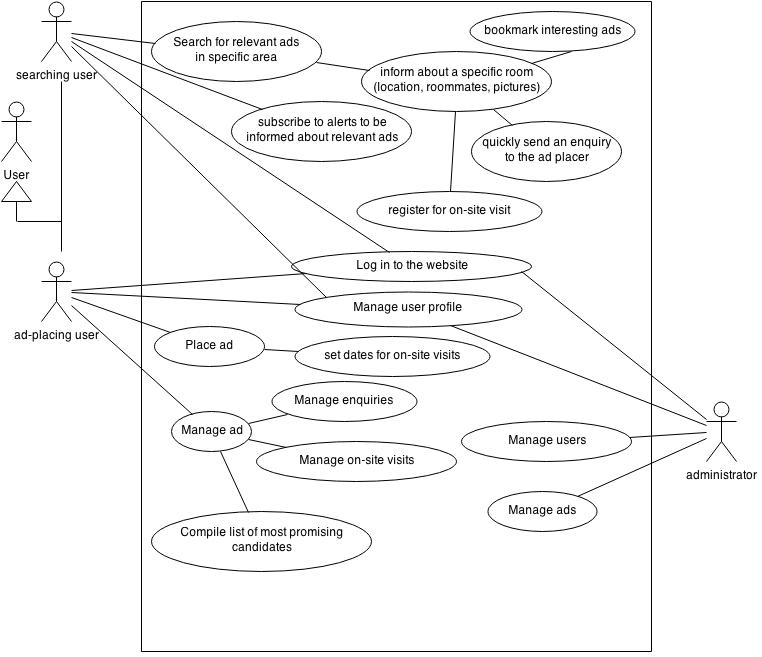
\includegraphics[width=0.8\textwidth]{Usecases}
\end{figure}
\end{center}
\subsection{Use cases}
\subsubsection{Search for relevant ads}
\begin{description}
\item[Actors] \mbox{}\\ Client; role: searching user.
\item[Description]\mbox{}\\
As a user, I want to search for relevant ads in a specific area.

\item[Trigger]\mbox{}\\
User starts filling in the search form.

\item[Pre-conditions]\mbox{}\\
User is logged in.

\item[Post-conditions]\mbox{}\\
User sees a list of relevant ads according to his search criteria
Search is persisted to database.
\item[Main scenario]\mbox{}\\
\begin{enumerate}
\item User indicates he wants to search for shared apartments.
\item User enters search area via zip code or map position and radius.
\item User enters price range.
\item User enters range of number of roommates
\item User enters preferred sex of roommates, if any.
\item User hits search button.
\item User sees list of relevant search results.
\end{enumerate}
\item[Alternative scenarios]\mbox{}\\
\textbf{1a.} User indicates he wants to search for normal apartments
\begin{enumerate}
\item Step 2 and 3 as in main scenario
\item User enters range for number of rooms
\item continue to step 6 of main scenario
\end{enumerate}
\textbf{3a.} User doesn't want to enter further details and hits the quick search button.
\begin{enumerate}
\item continue to step 7 of main scenario
\end{enumerate}
\textbf{7a.} After seeing the search results user wants to change his search criteria
\begin{enumerate}
\item User hits “change search criteria” button
\item User changes the desired criteria
\item continue to step 6 of main scenario
\end{enumerate}
\item[Notes]\mbox{}\\
Other search criteria? eg.: free from..., pre-defined keywords: vegetarian, rural, shared garden,...
\end{description}
\subsubsection{See room/apartment information}
\begin{description}
\item[Actors]\mbox{}\\
Client; role: searching user.

\item[Description]\mbox{}\\
As a user, I want to get exhaustive information about a room.

\item[Trigger]\mbox{}\\
User clicks on interesting ad, either after doing a search, or after opening list of bookmarked ads.

\item[Pre-conditions]\mbox{}\\
User is logged in.

\item[Post-conditions]\mbox{}\\
User sees room/apartment information

\item[Main scenario]\mbox{}\\
\begin{enumerate}
\item User sees the following:    
\begin{itemize}
\item map with indication of apartment location
\item pictures of the apartment/room details (price, …)
\item room/apartment description
\item link to roommates profiles
\end{itemize}
\item User can choose to sign up for an on-site visit, or to send an inquiry (depending on what the ad-placer allowed) or to bookmark the ad
\item User can go back to search results.
\end{enumerate}
\item[Notes]\mbox{}\\
Do we want to show short user profiles of the roommates or just a link to the roommate profiles?
\end{description}
\subsubsection{Bookmark ads}
\begin{description}
\item[Actors]\mbox{}\\
Client; role: searching user.
\item[Description]\mbox{}\\
As a user I want to bookmark interesting ads
\item[Trigger]\mbox{}\\
User clicks bookmark ad option when viewing an ad.
\item[Pre-conditions]\mbox{}\\
User is logged in.
\item[Post-conditions]\mbox{}\\
User gets a message that the ad is bookmarked.

List of bookmarked ads of user is updated.

In case of an error, or the user has already bookmarked this ad previously, a message stating this appears.
\item[Main scenario]\mbox{}\\
\begin{enumerate}
\item ad is bookmarked, message appears.
\end{enumerate}
\item[Alternative scenarios]\mbox{}\\
\textbf{1a.} couldn’t bookmark the ad because ad is already bookmarked.
\begin{enumerate}
\item ad already bookmarked message appears.
\end{enumerate}
\textbf{1b.} User realises he has bookmarked the wrong ad
\begin{enumerate}
\item User goes to my bookmarks
\item User clicks delete button next to the bookmark that has to be deleted
\end{enumerate}
\end{description}
\subsubsection{Subscribe to search alert}
\begin{description}
\item[Actors]\mbox{}\\
Client; role: searching user.
\item[Description]\mbox{}\\
As a user I want to subscribe to alerts to be informed about relevant ads.
\item[Trigger]\mbox{}\\
User hits search-alert button at the end of the search form.
\item[Pre-conditions]\mbox{}\\
User is logged in.

User Has filled in at least some search criteria in the form.
\item[Post-conditions]\mbox{}\\
Search criteria are linked to user profile in the database. 

User sees a success message.
\item[Main scenario]\mbox{}\\
\begin{enumerate}
\item User clicks search-alert button after filling in search form, or after viewing the list of ads corresponding to his search.
\item User can review search criteria
\item User hits save button
\item User sees search successfully saved message
\end{enumerate}
\item[Alternative scenarios]\mbox{}\\
\textbf{2a.} User notices a mistake in search criteria
\begin{enumerate}
\item User hits edit search criteria
\item User corrects mistake
\item Continue with step 3
\end{enumerate}
\end{description}
\subsubsection{send enquiry}
\begin{description}
\item[Actors]\mbox{}\\
Client; role: searching user.
\item[Description]\mbox{}\\
As a user I want to quickly send an inquiry to the ad-placer.
\item[Trigger]\mbox{}\\
User views an interesting ad, and clicks the send inquiry button.
\item[Pre-conditions]\mbox{}\\
User is logged in.

Ad placer has enabled searchers to send him a message.
\item[Post-conditions]\mbox{}\\
Message has been send by email to the ad placer.

Message is persisted to database.

User sees message send screen.
\item[Main scenario]\mbox{}\\
\begin{enumerate}
\item User clicks on send inquiry button
\item User enters his message.
\item User clicks send button
\item User views succes message.
\end{enumerate}
\item[Notes]\mbox{}\\
Does the user need to be able to edit his message after it has been send?
\end{description}
\subsubsection{Register for on-site visit}
\begin{description}
\item[Actors]\mbox{}\\
Client; role: searching user.
\item[Description]\mbox{}\\
As a user I want to register for an on-site visit.
\item[Trigger]\mbox{}\\
User is viewing an ad and hits register for visit button.
\item[Pre-conditions]\mbox{}\\
User is logged in.

Ad placer has opened some timeslots for on-site visits.

Not all timeslots are completely full yet.

User has not yet registered for a visit of this apartment
\item[Post-conditions]\mbox{}\\
User is registered for a time slot (in database)

Number of free places for timeslot is reduced by one.

User cannot register for other timeslots.

User has received a confirmation email.

\item[Main scenario]\mbox{}\\
\begin{enumerate}
\item User hits register for on-site visit button.
\item User sees open time slots and selects one.
\item User clicks register button
\end{enumerate}
\item[Alternative scenarios]\mbox{}\\
\textbf{2a.} User sees that he cannot attend any of the free timeslots
\begin{enumerate}
\item User cancels registration 
\item If ad placer has opened possibility to send inquiry, user can send an enquiry instead.
\end{enumerate}
\item[Notes]\mbox{}\\
Should unregistering be possible?
\end{description}
\subsubsection{Place ad}
\begin{description}
\item[Actors]\mbox{}\\
Client, role: ad-placing user

\item[Description]\mbox{}\\
As a ad-placing user I want to place an ad for the shared apartment.
\item[Trigger]\mbox{}\\
User triggers the “My Ads” button

\item[Pre-conditions]\mbox{}\\
Customer is logged in

\item[Post-conditions]\mbox{}\\
Ad saved in the data base.

User sees his ad and a confirmation

\item[Main scenario]\mbox{}\\
\begin{enumerate}
\item User enters the “My Ads” page, which contains a list of the already placed ads.
\item User pushes the “new” button
\item User fills in the data relevant for the living community.
\item User uploads pictures.
\item User indicates he wants to allow interessants to send an enquiry message
\item User saves the data.
\item User sees the ad as it would appear on the website and clicks the “confirm” button.
\item User will be directed to the “My Ads” page as in 1.
\end{enumerate}
\item[Alternative scenarios]\mbox{}\\
\textbf{5a.} User wants to set timeslots for visits instead
\begin{enumerate}
\item Step 6 as in main scenario
\item User enters user case 9.
\end{enumerate}
\textbf{6a.} User saved form with invalid data.
\begin{enumerate}
\item User gets an info of the incorrect insertion.
\item Use case resumes on step 3.
\end{enumerate}
\textbf{7a.} User sees ad and realizes he wrote something wrong.
\begin{enumerate}
\item User pushes the “Edit” button
\item Use case resumes on step 3
\end{enumerate}
\item[Special requirements]\mbox{}\\
User can only place a certain number of ads. (otherwise abuse has to be assumed)
\item[Notes]\mbox{}\\
Maximum size of ads per user?
\end{description}
\subsubsection{Set visiting dates}
\begin{description}
\item[Actors]\mbox{}\\
ad-placing user

\item[Description]\mbox{}\\
As ad-placing user I want to set dates for on-site visits so that searching users know when they can visit the flat.
\item[Trigger]\mbox{}\\
User has selected “set timeslots where interessants can register for visits” in the ad placing form and clicked  “Save”

OR

User clickes “add more timeslots” button next to a previously placed ad in the “My Ads” page.

\item[Pre-conditions]\mbox{}\\
User is logged in.

User has placed an ad.

\item[Post-conditions]\mbox{}\\
on-site visit dates are linked to ad in database

Ad-placing user sees the new dates

\item[Main scenario]\mbox{}\\
\begin{enumerate}
\item User clicks button (see trigger).
\item User inserts the dates
\item User inserts time slots
\item User sets number of users per time slot
\item User clicks “save time slots”
\end{enumerate}
\item[Alternative scenarios]\mbox{}\\
\textbf{1a.}  User has not placed any ad.
\begin{enumerate}
 \item User gets the information that no ad has placed yet.
\end{enumerate}
\textbf{5a.} User inserts an invalid date.
\begin{enumerate}
\item User gets the information that the date is invalid.
\item Use case resumes on step 2
\end{enumerate}
\end{description}
\subsubsection{Manage ad}
\begin{description}
\item[Actors]\mbox{}\\
Ad-placing user
\item[Description]\mbox{}\\
The ad-placing user wants to manage his ads.
\item[Trigger]\mbox{}\\
User clicks “my ads”-Button.
\item[Pre-conditions]\mbox{}\\
User logged in

User has created an ad

\item[Post-conditions]\mbox{}\\
User sees changed ad

Changes are persisted to the database
\item[Main scenario]\mbox{}\\
\begin{enumerate}
\item Clicks “my ads”-Button.
\item Clicks on the ad he wants to edit
\item Changes ad content
\item Clicks the save button
\item Sees the changed ad
\end{enumerate}
\item[Alternative scenarios]\mbox{}\\
\textbf{2a.} User wants to delete the ad
\begin{enumerate}
\item Clicks the delete button next to the ad.
\item User confirms the deletion
\item Ad is deleted and user is redirected to my ads page
\end{enumerate}
\end{description}
\subsubsection{Manage enquiries}
\begin{description}
\item[Actors]\mbox{}\\
Ad-placing user

\item[Description]\mbox{}\\
As a user I want to manage the enquiries.
\item[Trigger]\mbox{}\\
User clicks the enquiries button next to the ad in the “my ads” page.
\item[Pre-conditions]\mbox{}\\
User is logged in

Enquiries stack is not empty.

\item[Post-conditions]\mbox{}\\
\item[Main scenario]\mbox{}\\
\begin{enumerate}
\item User clicks the “enquiries” button.
\item User sees list of messages, including a sender profile picture a reply and delete button next to each message.
\item User reads message.
\item User double clicks on sender profile picture to see the complete profile of the candidate
\item User clicks back to go back to the enquiries 
\item User clicks reply
\item User writes a reply message
\item User clicks send
\end{enumerate}
\item[Alternative scenarios]\mbox{}\\
\textbf{6a.} User wants to delete the enquiry
\begin{enumerate}
\item User clicks delete button.
\end{enumerate}
\end{description}
\subsubsection{Manage on-site visits}
\begin{description}
\item[Actors]\mbox{}\\
Ad-placing user
\item[Description]\mbox{}\\
As a user I want to see how the timeslots I opened for flat visits are being filled up
\item[Trigger]\mbox{}\\
User clicks the “visiting times” button next to the ad in the my ads page.
\item[Pre-conditions]\mbox{}\\
user logged in
\item[Post-conditions]\mbox{}\\
Visiting dates and registered users are shown
\item[Main scenario]\mbox{}\\
\begin{enumerate}
\item Clicks the “visiting times” button.
\item User sees a list of opened timeslots and registered candidates. 
\item User can click on candidates names to see their full profile
\item User goes back to “visiting times” page
\end{enumerate}
\item[Alternative scenarios]\mbox{}\\
\textbf{3a.} User can click add more timeslots if he sees that only little places are left
\begin{enumerate}
\item User enters user case 9
\end{enumerate}
\textbf{3b.} User can change the number of allowed visitors for each timeslots as long as it does not go below the number of already registered candidates.
\begin{enumerate}
\item User changes the number
\item User clicks save changes button.
\end{enumerate}
\textbf{3c.} User can delete a timeslot completely, sending already registered users a message that the timeslot is deleted and that they can contact the ad placer or register for another timeslot.
\begin{enumerate}
\item User clicks delete button next to timeslot.
\item User confirms deletion
\item An automatic message to already registered users is compiled.
\end{enumerate}
\end{description}
\subsubsection{Compile list of promising candidates}
\begin{description}
\item[Actors]\mbox{}\\
Ad-placing user
\item[Description]\mbox{}\\
As a customer I want to compile a list of most compromising candidates.
\item[Trigger]\mbox{}\\
User clicks on “Candidates” button next to ad in “My Ads” page
\item[Pre-conditions]\mbox{}\\
 User logged in
 
 At least one candidate has registered for a visit or sent an enquiry.
\item[Post-conditions]\mbox{}\\
Changes are persisted to the database
\item[Main scenario]\mbox{}\\
\begin{enumerate}
\item User clicks on “Candidates” button
\item User sees a list of all candidates that have somehow reacted on the ad 
\item User can click through to see full candidate profile
\item User check “favorite” box next to his favorite candidates
\item User can click “compile favorite list” at the top of the page to see a shortlist of favorite candidates. 
\end{enumerate}
\end{description}
\subsubsection{Log in to the website}
\begin{description}
\item[Actors]\mbox{}\\
Ad-placing user, searching user, administrator
\item[Description]\mbox{}\\
The users want to have a profile with which to manage contact data and ads.
\item[Trigger]\mbox{}\\
Login is mandatory, so upon visiting the website, the user clicks the “Login” link.
\item[Pre-conditions]\mbox{}\\
None.
\item[Post-conditions]\mbox{}\\
User or administrator is logged in
\item[Main scenario]\mbox{}\\
\begin{enumerate}
\item Actor clicks the “Login” link.
\item The Persona login page opens and the user logs in.
\item The user is redirected to their profile page.
\end{enumerate}
\item[Alternative scenarios]\mbox{}\\
\textbf{3a.} The user has logged in for the first time, and after redirect is asked to choose a user name (and, depending on requirements, further information).
\end{description}
\subsubsection{Manage user profile}
\begin{description}
\item[Actors]\mbox{}\\
All users
\item[Description]\mbox{}\\
As a user, I want to be able to change my contact information, password, as well as manage my alerts, ads and favourites.

\item[Trigger]\mbox{}\\
User clicks the “Profile” link on the page.

\item[Pre-conditions]\mbox{}\\
The user is logged in.
\item[Post-conditions]\mbox{}\\
The data changed by the user is persisted to the DBMS.

The user is notified about the saved changes, or if it failed, why it did so.

\item[Main scenario]\mbox{}\\
\begin{enumerate}
\item Actor clicks the “Profile” link.
\item On the profile page, they can change their account data, ads, subscriptions and favourites.
\item Upon clicking “Save” the data gets stored if valid, and the user gets a notification about it on the profile page itself.
\end{enumerate}
\item[Alternative scenarios]\mbox{}\\
\textbf{2a.} If the user deletes their account, they get redirected to the main page.
\end{description}
\subsubsection{Manage users}
\begin{description}
\item[Actors]\mbox{}\\
The administrator.
\item[Description]\mbox{}\\
The administrator wants to be able to see all user data, and be able to delete and change users.

\item[Trigger]\mbox{}\\
The administrator clicks the “Admin panel” link next to the “Profile” link.
\item[Pre-conditions]\mbox{}\\
The user is logged in

The user is marked as administrator

\item[Post-conditions]\mbox{}\\
The changes are persisted to the database if they’re valid

The admin gets notified about that

\item[Main scenario]\mbox{}\\
\begin{enumerate}
\item Administrator clicks on “Admin panel” link
\item The admin searches for a user using the admin panel search function
\item The admin selects a user from the user list
\item The user’s profile page is displayed, where the admin can change the user’s data and settings, as well as delete the user
\item After all changes are done, the admin leaves the page
\end{enumerate}

\end{description}
\subsubsection{Manage ads}
\begin{description}
\item[Actors]\mbox{}\\
The administrator
\item[Description]\mbox{}\\
As administrator, I want to be able to change ads on behalf of users, and delete ads for a number of reasons.
\item[Trigger]\mbox{}\\
The administrator clicks the “Admin panel” link next to the “Profile” link.
\item[Pre-conditions]\mbox{}\\
The user is logged in

The user is marked as administrator
\item[Post-conditions]\mbox{}\\
The changes are persisted to the database if they’re valid

The admin gets notified about that

\item[Main scenario]\mbox{}\\
\begin{enumerate}
\item Admin clicks on “Admin panel” link
\item The admin first searches for a user (as described in scenario 16, “Manage users”), then selects an ad from that user’s list of ads
\item The admin selects an ad from the ad list
\item The admin searches for an ad using the admin panel search function
\item On the ad management panel (the same as for the ad-placing user) the admin can change all data, as well as delete the ad
\item After all changes are done, the admin leaves the page

\end{enumerate}
\end{description}
\subsection{Actor Characteristics}
All users are logged in and have a minimal user profile (name, email address,...)

The clients of our website are people looking for a (shared) apartment in Switzerland.
The main user group will be between aged 18 - 29 years old. 
We expect most but not all apartments to be in and around univeristy cities.
These users can place ads for (shared) apartments or search the ads. 
We expect these group of users to be the largest group of actors.

Another actor group is the administrator group. This is a small group of 1 to 5 people, who can view all information about users and ads. Members of this group are permitted by our customer. 


\end{document}
